\documentclass[../ECE459FinalProjectReport.tex]{subfiles}

\begin{document}
\chapter{Methodology}
This chapter presents the methodology employed in the project using Python 3. The simulations were executed within the Jupyter Notebook environment, leveraging essential packages for numerical computation, signal analysis, and plotting, namely \verb|numpy|, \verb|scipy|, and \verb|matplotlib|.

\section{Choice of Message Signal}

Two distinct message signals were selected for thorough investigation in this project:
\begin{enumerate}
    \item The multi-tone sinusoidal signal $m_1 (t) = A_1\cos(2\pi f_1 t + \phi_1) + A_2 \cos(2\pi f_2 t + \phi_2)$.
    \item The TTS-generated recording of a male voice reading ``ECE 459 is so interesting.''
\end{enumerate}

The first signal, a multi-tone sinusoidal waveform, was chosen for its simplicity as a periodic function and its unique attributes as a linear combination of two sinusoidal functions. This particular choice facilitates the observation of distortion induced by noise, given the relatively straightforward frequency spectra of sinusoidal functions. 

The utilization of a TTS-generated male voice recording, on the other hand, introduces a more realistic scenario, allowing the team to experiment with the designed communication system in a practical context. Such recording has no background noise between words, which enables the team to better observe the distortion by the simulated noise process.

\section{Additive White Gaussian Noise}
Additive White Gaussian Noise (AWGN) refers to a Gaussian process that can be directly added to a signal to approximate a noise-distorted signal in a real-life communication channel.

According to \cite[Sec. 8.10]{haykinIntroductionAnalogDigital2007}, a noise process is called white noise if it has zero mean and its power spectral density satisfies
\begin{equation}
    S_W(f) = \frac{N_0}{2}.
\end{equation}

The power spectrum of a white noise process is shown in Figure \ref{fig:white-noise-spectrum}.
\begin{figure}[htb]
    \centering
    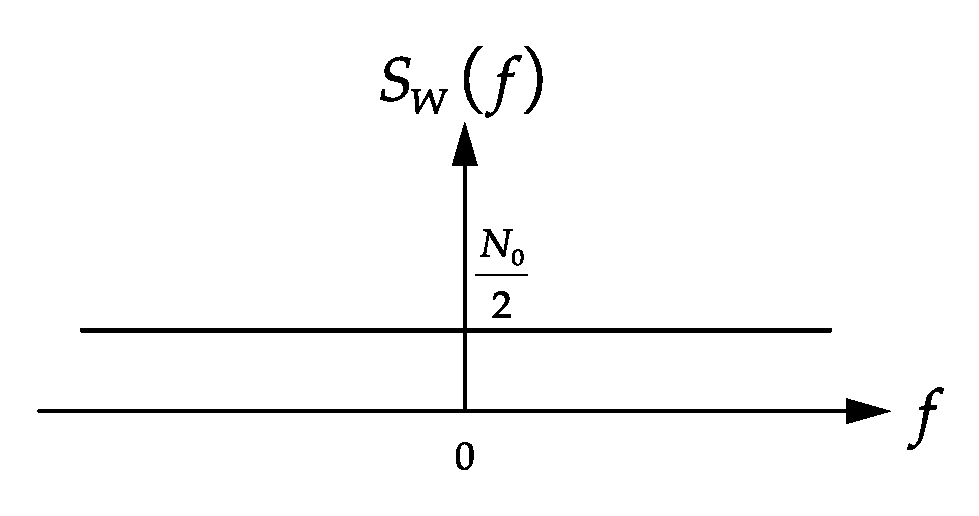
\includegraphics[scale=0.4]{plots/white-noise-power-spectrum.pdf}
    \caption{The power spectrum of a white noise process.}
    \label{fig:white-noise-spectrum}
\end{figure}

%todo: 写一下Python产生的Gaussian过程+功率谱

\section{AM Simulation}
\subsection{Envelope Modulation}
%?? What about transmission bandwidth??
Consider a message signal $m(t)$ and carrier wave $A_c \cos(2\pi f_c t + \phi)$ where $\phi$ is the phase delay of the local oscillator. In this project, we pick $\phi = 0$ for simplicity. The modulation of a message signal, denoted as $m(t)$, can be achieved through envelope modulation, represented by the equation:
\begin{equation}
    s(t) = A_c [1 + k_a m(t)] \cos (2\pi f_c t + \phi)
\end{equation}
In this expression, $k_a$ denotes the modulation sensitivity, $A_c$ corresponds to the amplitude of the carrier wave, and $f_c$ represents the frequency of the carrier wave. It is imperative to ensure that the carrier wave frequency $f_c$ significantly surpasses the highest frequency component, denoted as $W$, of the message signal $m(t)$ to prevent aliasing. This condition can be expressed as $f_c \gg W$. Moreover, the choice of the modulation sensitivity, $k_a$, needs to adhere to the constraint which is crucial to prevent envelope distortion, as outlined by \textcite[pp. 101-102]{haykinIntroductionAnalogDigital2007}:
\begin{equation}
    \left| k_a m(t) \right| < 1, \quad \text{for all }t.
\end{equation}

The product of modulation sensitivity $k_a$ and amplitude of message signal $A_m$
\begin{equation}
    \mu = k_a A_m
\end{equation}
is called the modulation factor, or as stated by \cite{sasmitaModulationIndexModulation2020}, the \textit{modulation index}. It can be alternatively expressed as
\begin{equation}
    \mu = \frac{A_m}{A_c}.
\end{equation}
In this project, the AM modulation index is specified as $\mu=0.3$.

The implementation of amplitude modulation (AM) can be illustrated through the block diagram depicted in Figure \ref{fig:env-mod}. The message signal is amplified by a gain $k_a$ and is added a DC offset. The carrier wave is then multiplied with the scaled and shifted message signal, which produces the envelope-modulated wave that is to be transmitted through the channel.
\begin{figure}[b]
    \centering
    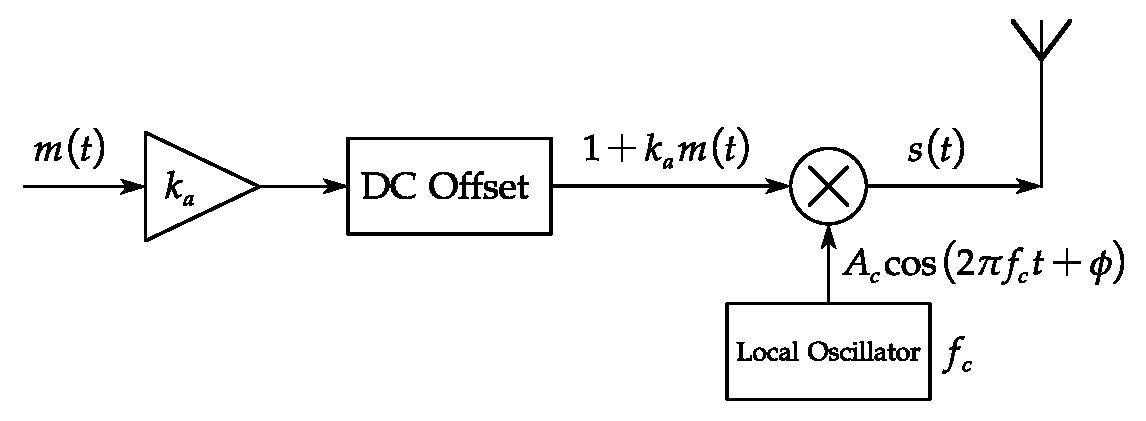
\includegraphics[scale=0.6]{plots/env_mod.pdf}
    \caption{Block diagram illustrating the process of envelope modulation.}
    \label{fig:env-mod}
\end{figure}

\subsection{Envelope Detection}
Diverging from coherent detection, envelope detection dispenses with the necessity of multiplying the received signal by the carrier wave. Instead, the received signal undergoes filtration by a Band Pass Filter (BPF) to eliminate noise beyond the desired bandwidth, and subsequently, an envelope detector facilitates the recovery of the message signal. This procedural sequence is depicted in Figure \ref{fig:env-demod}.

In physical circuitry, the envelope detector typically comprises a diode and an LPF \cite{AnalogCommunicationAM}. However, in Python, this functionality is realized through a Hilbert transform process \cite{ulrichEnvelopeCalculationHilbert2006, XiXiaoShengPythonTiQuXinHaoDeBaoLuoGet2023}.

Consider a single-tone sinusoidal signal with frequency $f_m$ modulated by a carrier wave with frequency $f_c$. The modulated wave, denoted as $g(t)$, is expressed as
\begin{equation}
    g(t) = \sin(2\pi f_c t)\sin(2\pi f_m t)
\end{equation}
where $f_c\gg f_m$. By trigonometric identity, $g(t)$ can be alternatively expressed as
\begin{equation}
    g(t)=-\frac{1}{2}\{\cos\mathrm[2\pi (f_c+f_m)t]-\cos[2\pi (f_c-f_m)t]\}.
\end{equation}

The Hilbert transform introduces a $-\frac{\pi}{2}$ to the phase of the signal, which yields
\begin{equation}
    \begin{aligned}
        \tilde{g}(t)&=-\frac{1}{2}\left\lbrace\cos\left[2\pi (f_c+f_m)t - \frac{\pi}{2}\right]-\cos\left[2\pi (f_c-f_m)t - \frac{\pi}{2}\right]\right\rbrace\\
        &=-\frac{1}{2}\left\{ \sin\left( 2\pi f_ct-\frac{\pi}{2} \right) \sin\left( 2\pi f_mt \right) \right\} \\
                    &=-\frac{1}{2}\cos\left( 2\pi f_ct \right) \sin\left( 2\pi f_mt \right) 
    \end{aligned}
\end{equation}

The analytic signal of $g(t)$, denoted as $\aleph\{g(t)\}$, can be expressed as a combination of $g(t)$ and its Hilbert transform $\tilde{g}(t)$, which is
\begin{equation}
    \aleph\{g(t)\} = g(t) + j\tilde{g}(t) = \sin(2\pi f_c t)\sin(2\pi f_m t) - j\cos(2\pi f_c t)\sin(2\pi f_m t).
\end{equation}

The magnitude of the analytic signal can be calculated by
\begin{equation}
    \left| \aleph\{g(t)\}\right| = \sqrt{\aleph\{g(t)\}\aleph^*\{g(t)\}} = \left| \sin(2\pi f_m t)\right|
\end{equation}
which precisely equals to the original $g(t)$.

Thus, the envelope of an envelope-modulated signal can be derived by calculating the magnitude of the Hilbert transform of the signal,
\begin{equation}
    \text{envelop of $s(t)$} = \left| \tilde{s}(t) \right|
\end{equation}
where $\tilde{s}(t)$ is the Hilbert transform of $s(t)$.

This methodology is applied by the team in the project.

\begin{figure}[htb]
    \centering
    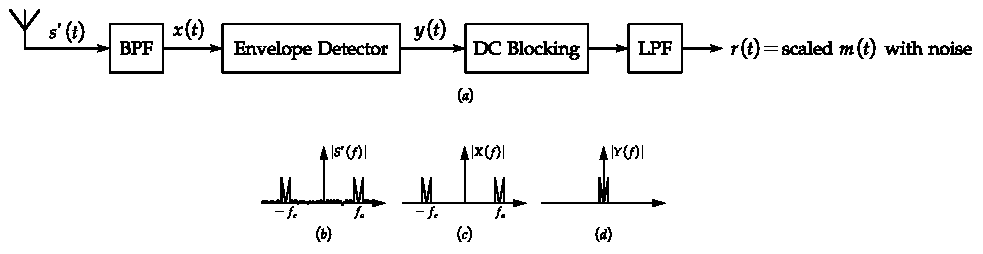
\includegraphics[width=\linewidth]{plots/env-demod.pdf}
    \caption{Block diagram illustrating the process of envelope demodulation.}
    \label{fig:env-demod}
\end{figure}

\subsection{SNR Calculation and Measurement}
\subsubsection{Pre-Detection SNR}
As is stated in \textcite[Eq. (9.26)]{haykinIntroductionAnalogDigital2007}, the theoretical pre-detection SNR in an envelope modulation receiver can be calculated by
\begin{equation}
  \SNR_{\text{pre, theoretical}}^{\text{AM}} = \frac{A_c^2 (1+k_a^2)P}{2N_0 B_T}
\end{equation}
where $A_c$ is the carrier amplitude, $k_a$ is the modulation sensitivity, $P$ is the power of message signal, $N_0$ is twice the power spectral density of white noise and $B_T$ is the noise bandwidth of the BPF.

Following the notation in Figure \ref{fig:env-demod}, the actual pre-detection SNR can be measured as
\begin{equation}
    \SNR_{\text{pre, measured}}^{\text{AM}} = \frac{\E[x(t)]}{\text{noise power}}.
\end{equation}

%todo:如何测量噪声?What exactly is ``noise power''??

\subsubsection{Post-Detection SNR}

The textbook \cite[Eq. (9.23)]{haykinIntroductionAnalogDigital2007} states that the theoretical post-detection SNR in an envelope modulation receiver is expressed as
\begin{equation}
    \SNR_{\text{post, theoretical}}^{\text{AM}} = \frac{A_c^2 k_a^2 P}{2N_0 W}
\end{equation}
which is a valid approximation only for high SNR and $0<k_a<100\%$.

The actual post-detection SNR can be expressed as, if following the notation in Figure \ref{fig:env-demod},
\begin{equation}
    \SNR_{\text{post, measured}}^{\text{AM}} = \frac{\E[y(t)]}{\text{noise power}}.
\end{equation}

%todo:如何测量噪声

\subsubsection{Relation between Pre- and Post-Detection SNRs}
%todo:考虑是否要找一下在高pre-detection SNR和低pre-detection SNR的情况下post-detection分别是什么关系,
%todo:书上有图9.12

\section{FM Simulation}
\subsection{Narrow-Band FM Modulation}
The textbook \cite[Sec. 4.1]{haykinIntroductionAnalogDigital2007} states that the message signal $m(t)$ will be phase-modulated with a carrier signal $A_c \cos(2\pi f_c t)$, which obtains the frequency modulated wave
\begin{equation}
    s(t) = A_c \cos\left[ 2\pi f_c t + 2\pi k_f \int_0^{t} m(\tau) \D\tau \right]
\end{equation}
where the instantaneous frequency is
\begin{equation}
    f_i(t) = f_c + k_f m(t).
\end{equation}
Here $k_f$ denotes the modulation sensitivity which determines the frequency deviation by
\begin{equation}
    \Delta f = k_f A_m.
\end{equation}

By Carson's rule, \cites[Sec. 4.6]{haykinIntroductionAnalogDigital2007}{CarsonRule2017}, the transmission bandwidth of an FM wave for a single-tone modulating wave is estimated as
\begin{equation}
    B_T = 2\Delta f + 2f_{m,\mathrm{max}}
\end{equation}
where $f_{m,\mathrm{max}}$ is the highest modulating frequency. The ratio of $\Delta f$ and $f_m$ is defined as modulation index,
\begin{equation}
    \beta = \frac{\Delta f}{f_m}.
\end{equation}
In this project, the modulation index is specified as $\beta=3$.

Such modulation can be done using a direct method \cite[Sec. 4.7]{haykinIntroductionAnalogDigital2007}, where the frequency modulator contains an oscillator directly controllable by the message signal. Figure \ref{fig:fm-mod} illustrates this process: the message signal is taken integral and sent to the controllable oscillator to produce a phase-variant signal, which is the modulated wave.


\begin{figure}[htb]
    \centering
    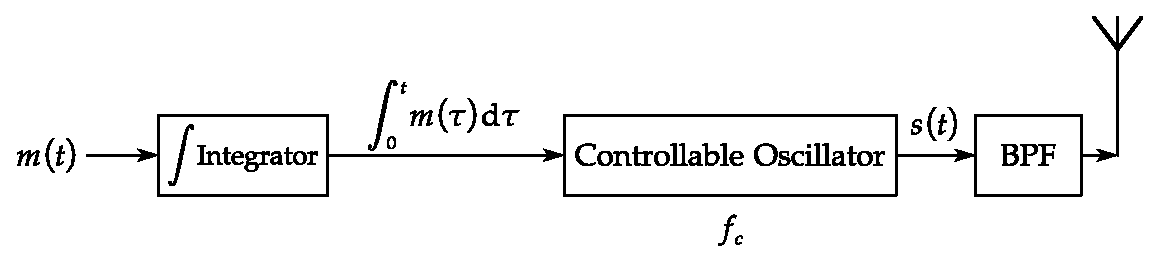
\includegraphics[scale=0.6]{plots/fm_mod.pdf}
    \caption{The direct method of narrow-band FM modulation.}
    \label{fig:fm-mod}
\end{figure}


\subsection{Narrow-Band FM Demodulation}
~
\subsection{SNR Calculation and Measurement}
~

\section{Filter Design}
\subsection{Ideal Filters}
%todo 讲LPF和BPF的TF,然后引出为什么ideal filter无法实现,再引出butterworth
~
\subsection{Butterworth Filter in Python}

Both Amplitude Modulation (AM) and Frequency Modulation (FM) communication systems necessitate the incorporation of filters. In practical scenarios, however, the realization of ideal filters poses inherent challenges. Nevertheless, the Butterworth Filter exhibits characteristics closely approximating those of an ideal filter. Figures \ref{fig:butter-lpf} and \ref{fig:butter-bpf} depict the frequency responses of Butterworth LPF and BPF with varying orders, illustrating that an increased order ($n$) results in a more pronounced roll-off slope. As expounded by \cite{storrButterworthFilterDesign2013, kudekiAnalogSignalsSystems2009}, a Butterworth Low Pass Filter manifests a maximally flat frequency response within its passband, swiftly attenuating beyond the cut-off frequency. This advantageous attribute empowers the design of filters with minimal distortion, albeit at the expense of an indeterminate phase delay induced by the inherent properties of Infinite Impulse Response (IIR) filters.

In the digital realm, Python facilitates the implementation of filters as digital IIR filters, with each filter in the $z$-domain expressed as the quotient of two polynomials:
\begin{equation}
H_{\text{filter}}(z) = \frac{\sum_{p=0}^{n}{a_pz^{-p}}}{\sum_{q=0}^{n}{b_qz^{-q}}}
\end{equation}

The response of the filter is uniquely determined by coefficients $a_i$ and $b_j$ ($0 \leq i, j \leq n$), where these coefficients can be computed using the \verb|scipy.signal.butter()| function, as documented by \cite{thescipycommunityScipySignalButter, thescipycommunityScipySignalFiltfilt, thescipycommunityScipySignalLfilter}. A practical instantiation of an IIR filter is exemplified below:
\begin{lstlisting}[language=python]
# Generate an 8-order 40 Hz to 80 Hz IIR BPF, sample rate = fs
b, a = butter(N=8, [40, 80], btype='band', fs=fs)
# Apply the filter to the message signal
filtered_signal = filtfilt(b, a, message)
\end{lstlisting}

Figures \ref{fig:butter-lpf} and \ref{fig:butter-bpf} showcase the frequency response of a Butterworth LPF and BPF, respectively, each featuring a cut-off frequency of $\omega_c = \SI{100}{\radian\per\s}$. The black dashed line denotes the \SI{-3}{\dB} amplitude.

\begin{figure}[htb]
    \centering
    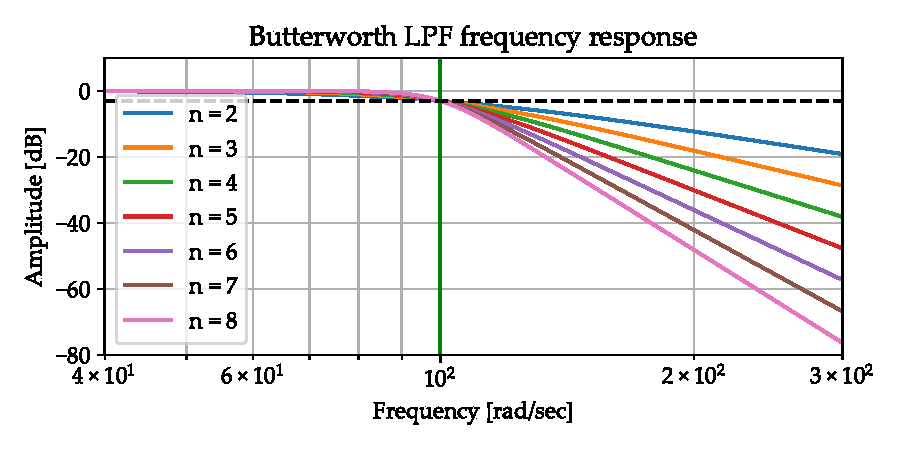
\includegraphics[width=0.45\linewidth]{plots/butterworth-lpf.pdf}
    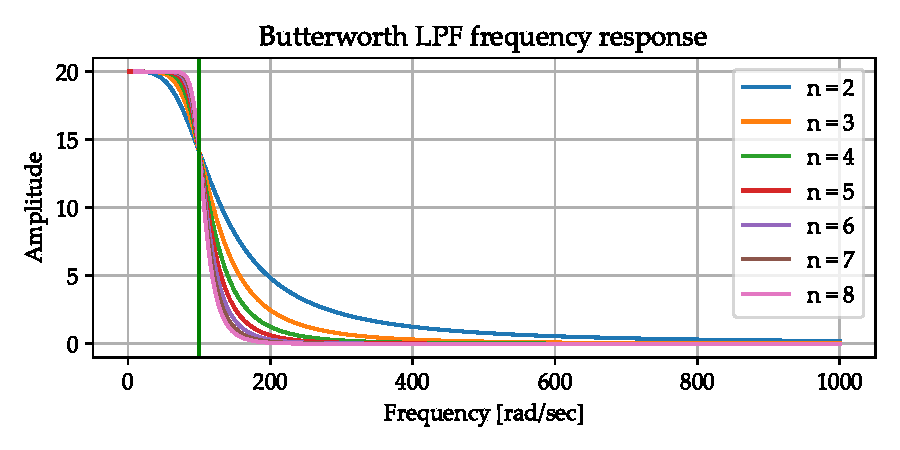
\includegraphics[width=0.45\linewidth]{plots/butterworth-lpf-nolog.pdf}
    \caption{The frequency response of a Butterworth LPF with cut-off frequency $\omega_c = \SI{100}{\radian\per\s}$. The black dash line shows the \SI{-3}{\dB} amplitude.}
    \label{fig:butter-lpf}
\end{figure}
\begin{figure}[htb]
    \centering
    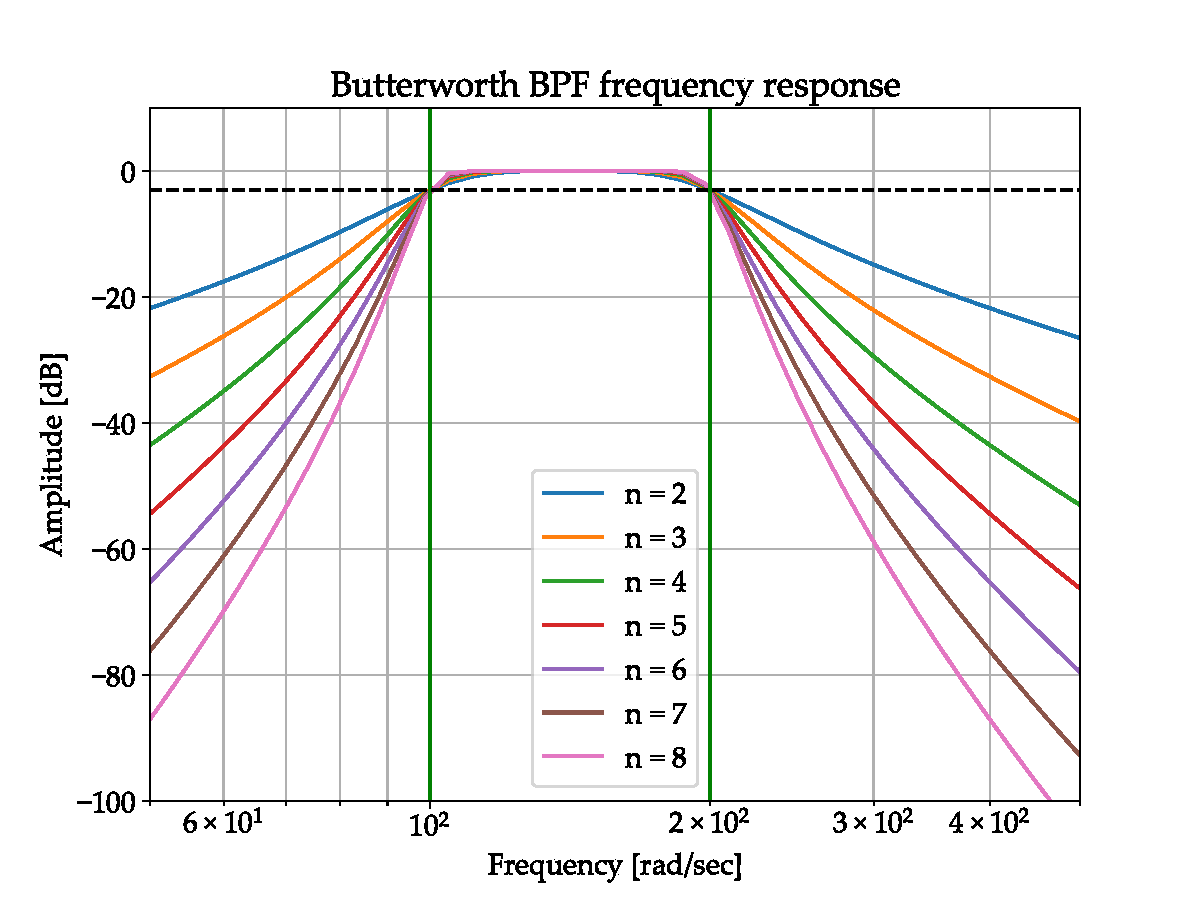
\includegraphics[width=0.45\linewidth]{plots/butterworth-bpf.pdf}
    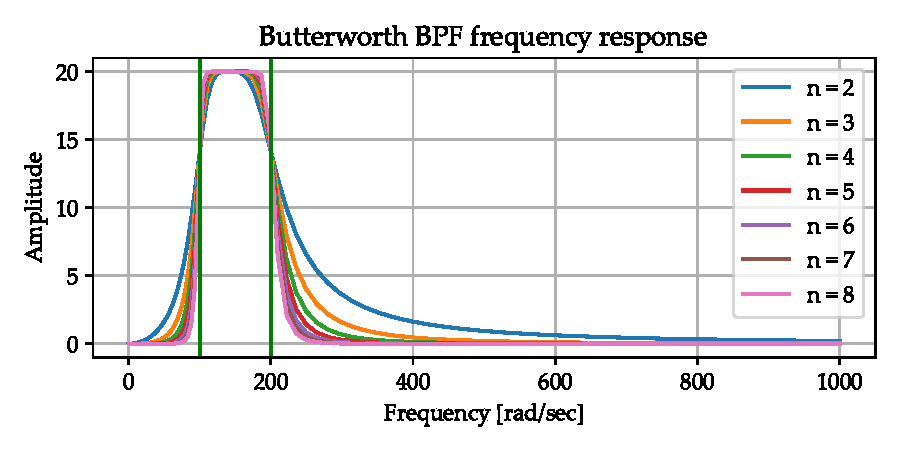
\includegraphics[width=0.45\linewidth]{plots/butterworth-bpf-nolog.pdf}
    \caption{The frequency response of a Butterworth BPF with pass-band from \SI{100}{Hz} to \SI{200}{Hz}. The black dash line shows the \SI{-3}{\dB} amplitude.}
    \label{fig:butter-bpf}
\end{figure}



\end{document}